\documentclass[10pt]{article}[H]
\usepackage{amsmath,amssymb}
\setlength{\oddsidemargin}{0in}
\setlength{\evensidemargin}{0in}
\setlength{\textheight}{9in}
\setlength{\textwidth}{6.5in}
\setlength{\topmargin}{-0.5in}
\usepackage{enumitem}
\usepackage{graphicx}
\usepackage{multirow}
\usepackage{float}
\usepackage{pdfpages}
\usepackage{subfigure}

\title{\bf Math 167: Homework 3}
\date{8/27/2023}
\author{\bf Owen Jones}

\begin{document}
\maketitle
\begin{itemize}
    \item [\textbf{Exercise 6.1}] We want to show by backwards induction that the optimal strategy to be greedy at every node. 
    Consider the node with pot size $99$. Player II has the options to be greedy and obtain $51$ leaving Player I with $48$ or continue and split the $100$ pot $50/50$. Since $51>50$, Player II should pick greedy. 
    Player I, anticipating Player II's next move, realizes they now have the choice between stealing $51$ from the pot size $98$ or continuing and allow Player II to be greedy on their next turn. 
    We now assume the next player will be greedy on their next turn for some arbitrary pot size $>4$. 
    Then, the current player chooses $\max\{\lfloor\frac{p+4}{2}\rfloor,(p+1)-\lfloor\frac{(p+1)+4}{2}\rfloor\}$ 
    If $p$ is even let $2q=p$. Then, $\lfloor\frac{p+4}{2}\rfloor=q+2>q-1=(p+1)-\lfloor\frac{(p+1)+4}{2}\rfloor$. 
    If $p$ is odd, let $2q+1=p$. Then $\lfloor\frac{p+4}{2}\rfloor=q+2>q-2=(p+1)-\lfloor\frac{(p+1)+4}{2}\rfloor$.
    In both cases, the current player obtains a better payoff by being greedy. 
    Hence, the pure equilibria are $(G,G)$ at every node. 
    \item [\textbf{Exercise 6.2}] Shown below are the Bayesian game tree and normal form of the game.
    \begin{figure}[H]
        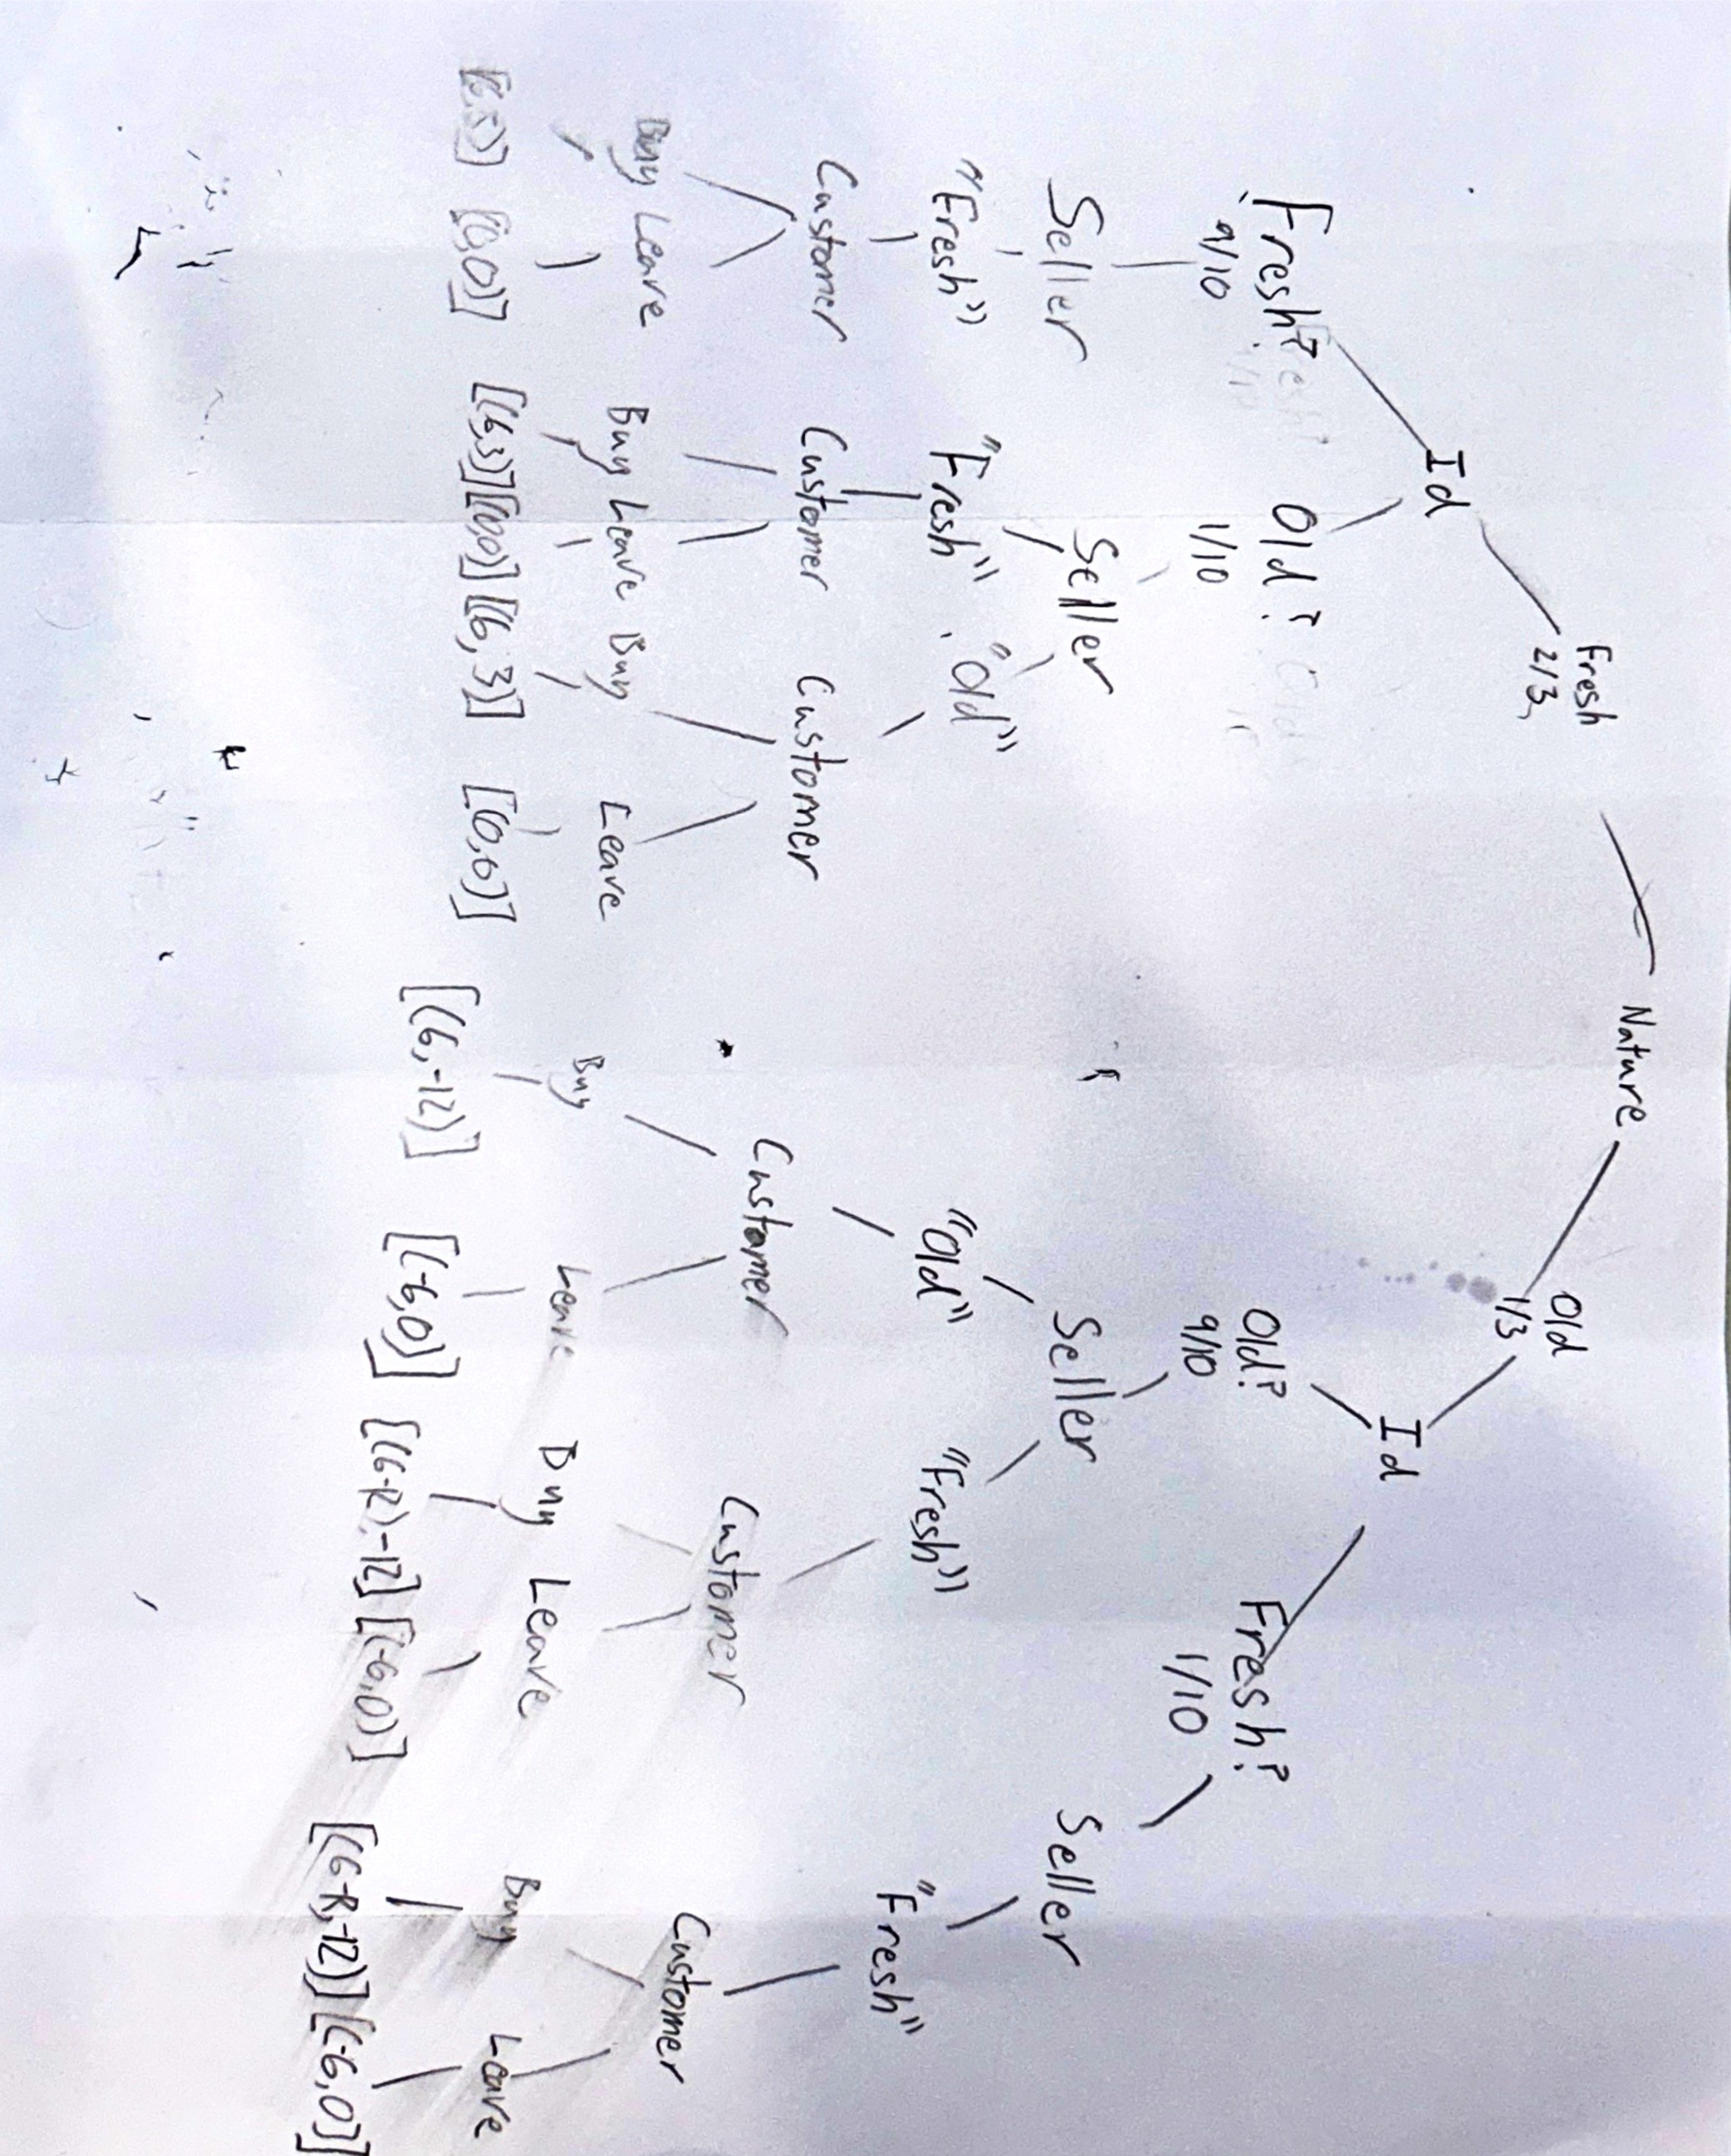
\includegraphics[scale=0.1, angle=90]{Tree_1.pdf}    
    \end{figure} 
    \begin{table}[H]
        \begin{tabular}{llll}
                               &                         & C                                                     &                             \\ \cline{2-4} 
        \multicolumn{1}{l|}{}  & \multicolumn{1}{l|}{}   & \multicolumn{1}{l|}{BL}                               & \multicolumn{1}{l|}{LL}     \\ \cline{2-4} 
        \multicolumn{1}{l|}{S} & \multicolumn{1}{l|}{OF} & \multicolumn{1}{l|}{(2-$\frac{R}{30}$,$\frac{7}{5}$)} & \multicolumn{1}{l|}{(-2,0)} \\ \cline{2-4} 
        \multicolumn{1}{l|}{}  & \multicolumn{1}{l|}{FF} & \multicolumn{1}{l|}{(6-$\frac{R}{3}$,-2)}             & \multicolumn{1}{l|}{(-2,0)} \\ \cline{2-4} 
                               &                         &                                                       &                             \\
                               &                         &                                                       &                            
        \end{tabular}
        \end{table}
    \item [\textbf{Exercise 6.3}] Below is the Bayesian game trees.
    \begin{figure}[H]
        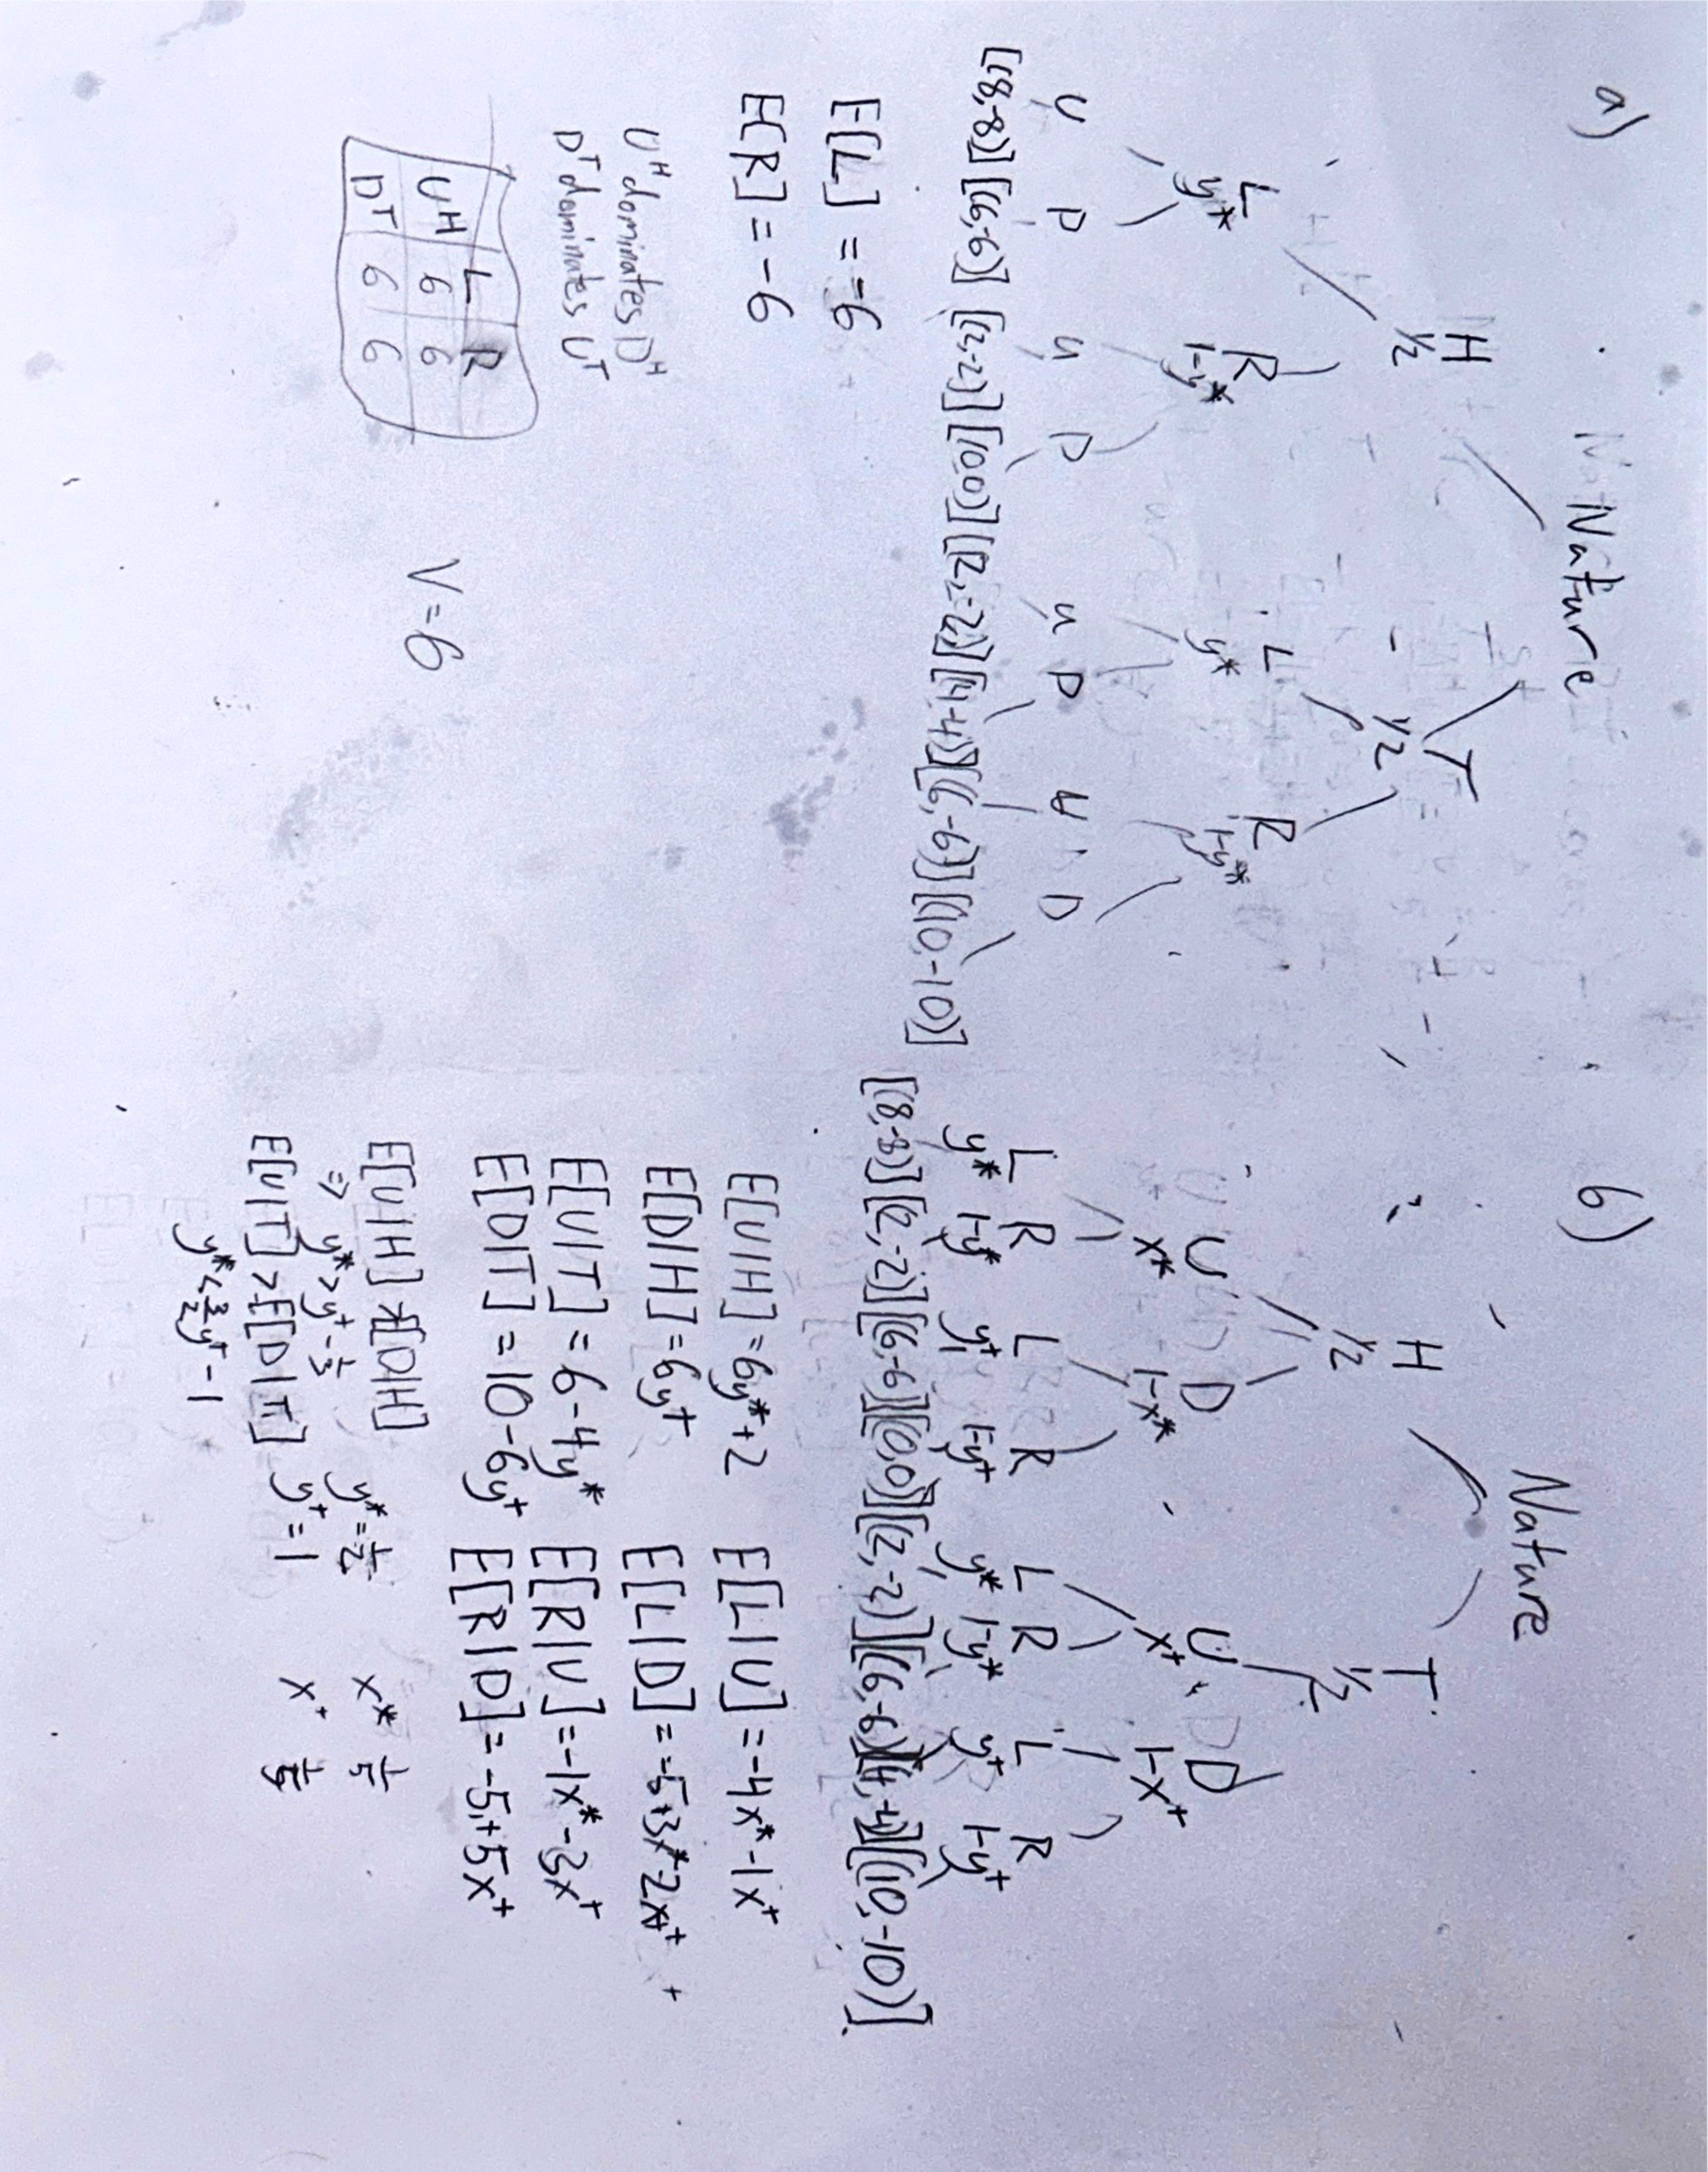
\includegraphics[scale=0.1, angle=90]{Tree_2.pdf}    
    \end{figure} 
    \item [\textbf{Exercise 6.4}] \begin{itemize}
        \item [PI=K] Bets with $P(B_1|K)=3\alpha$ for $\alpha\le\frac{1}{3}$. $E[K]=\frac{7}{6}$
        \item [PI=Q] Should always pass on first turn. Should call with $P(C_2|Q)=\frac{1}{3}$. $E[Q]=-\frac{1}{3}$
        \item [PI=J] Bets wit $P(B_1|J)=\alpha$. Should never call. $E[J]=-1$ Since $P(B_1|J)>0$ there is bluffing.
        \item [PII=K] Should always call in response to a bet and bets in response to a pass.
        \item [PII=Q] Should always pass in response to a pass and calls with $P(C_2|Q)=\frac{1}{3}$
        \item [PII=J] Should always fold in response to a bet and bets with $P(B_2|J)=\frac{1}{3}$
        \item Value of game for Player I is $-\frac{1}{18}$
    \end{itemize}
    \begin{figure}[H]
        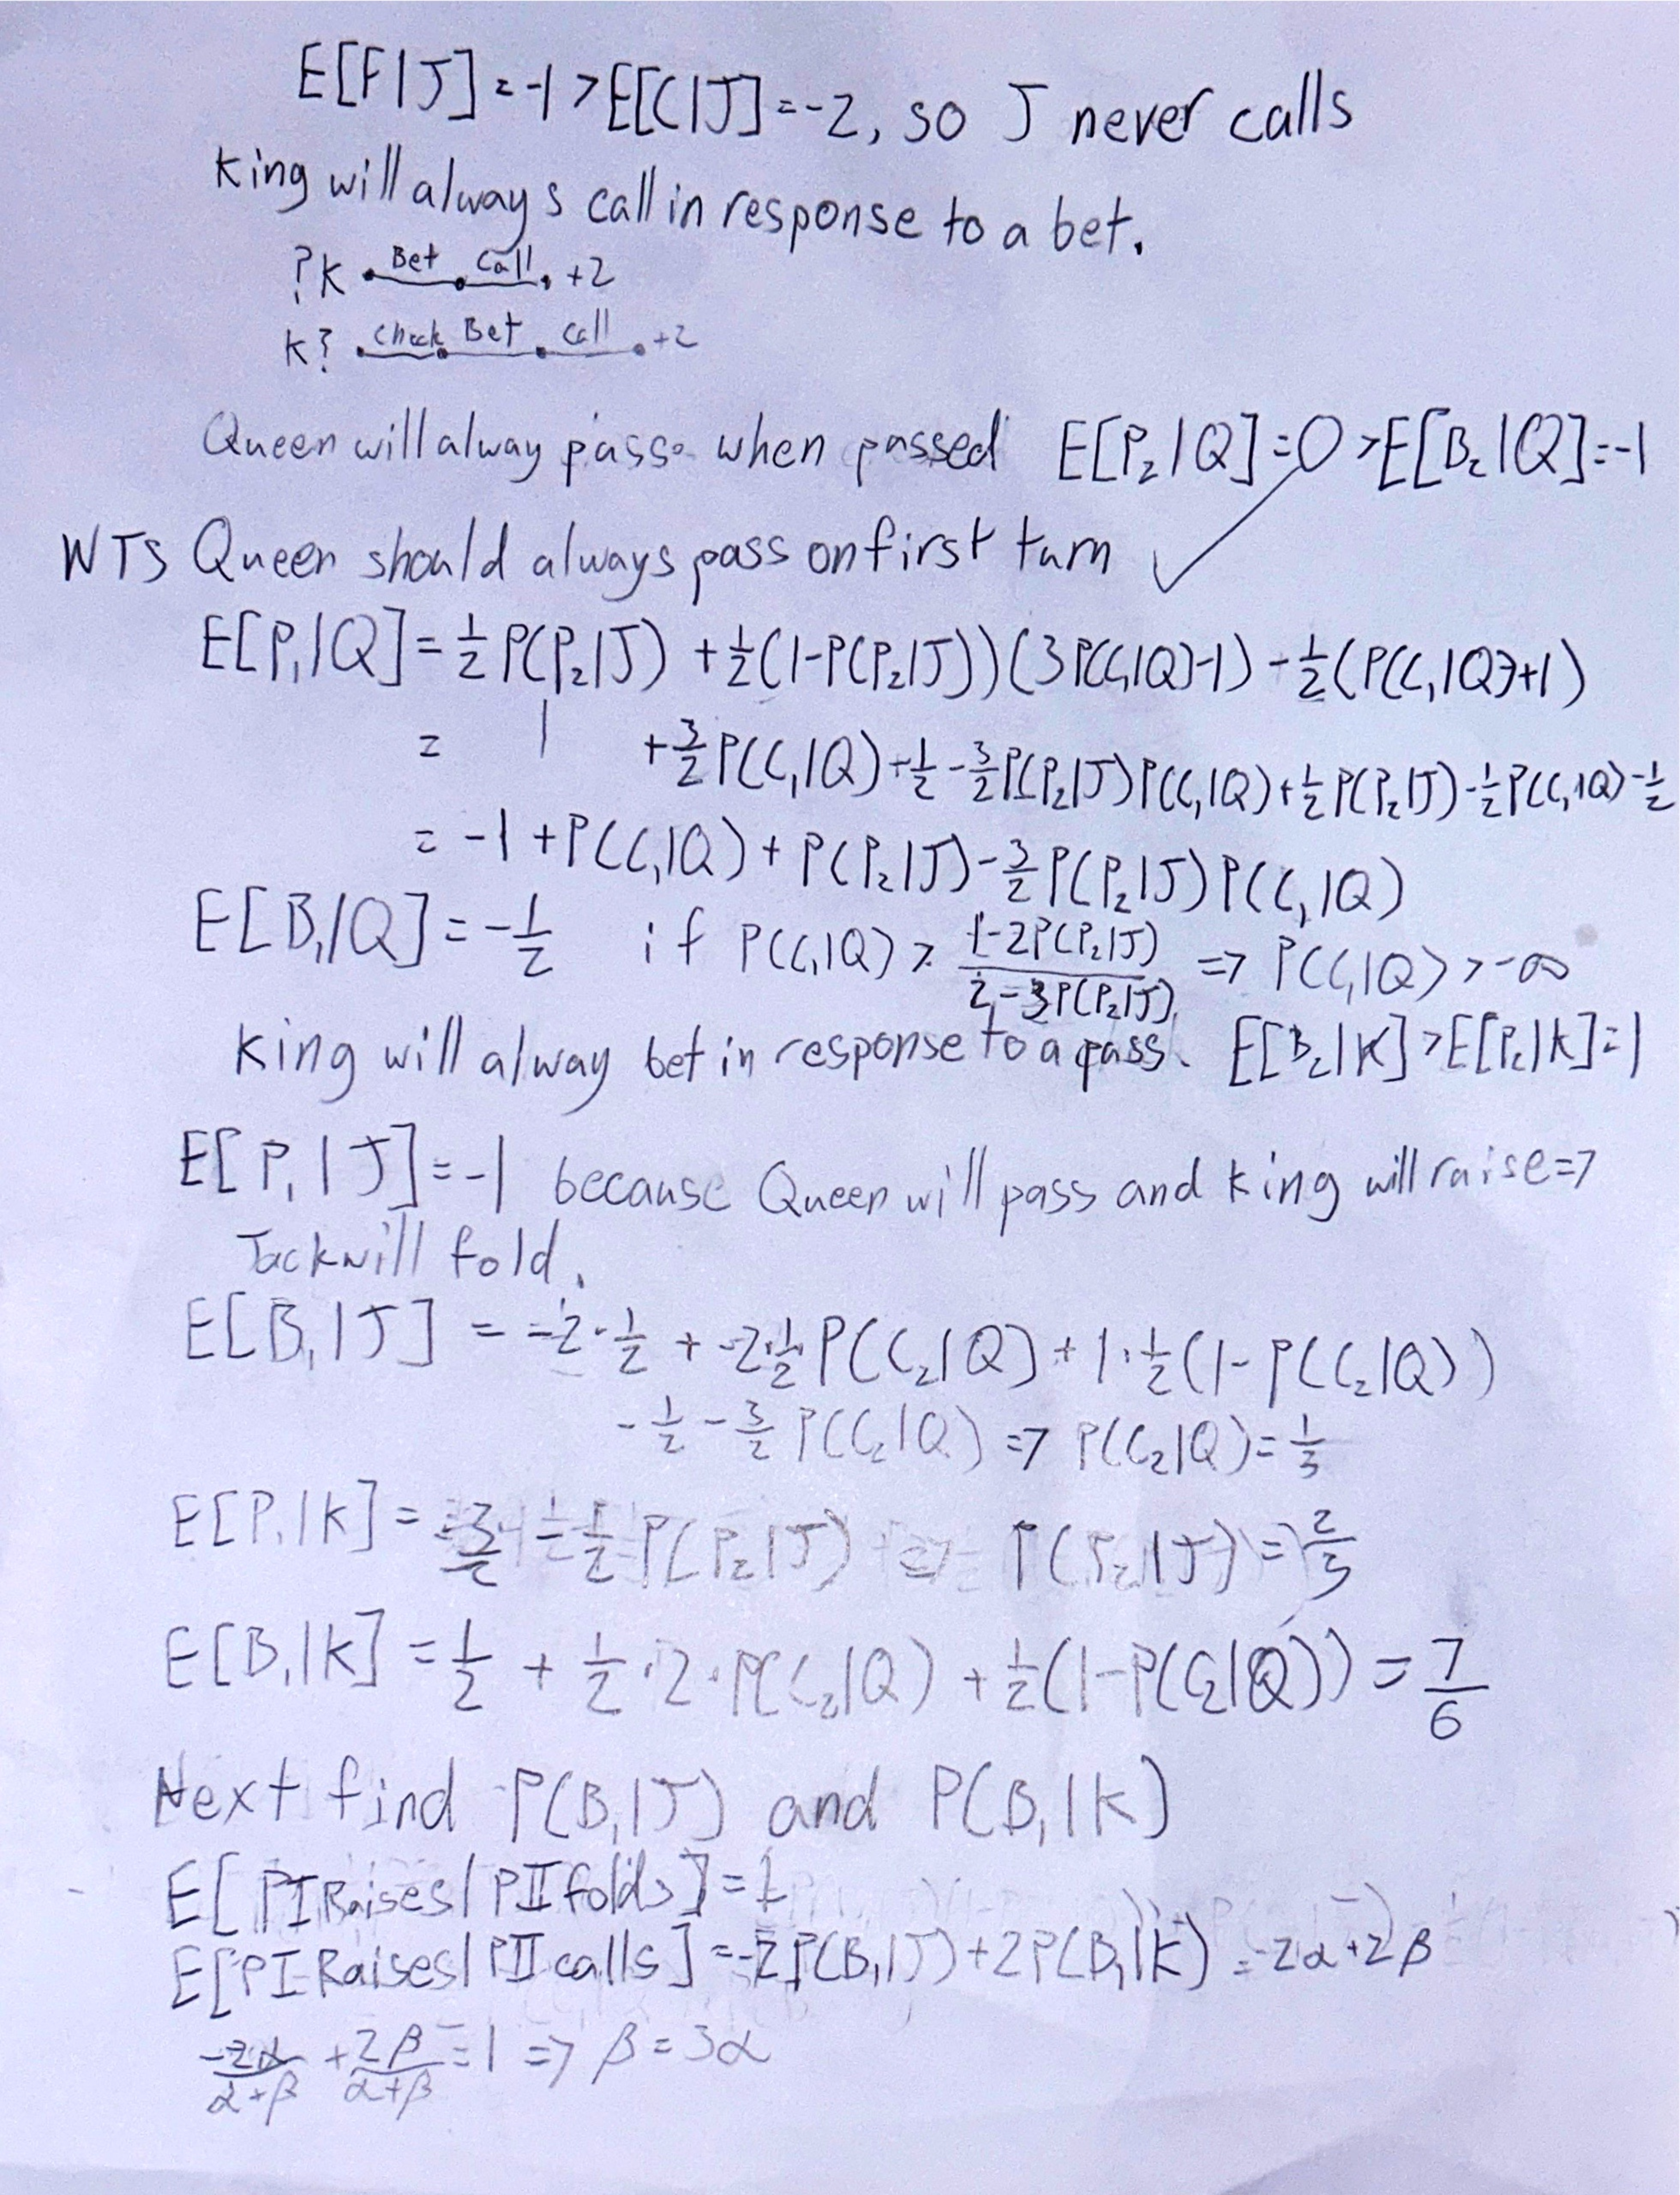
\includegraphics[scale=0.1,page=1]{6_4.pdf}
        \includegraphics[scale=0.1,page=2]{6_4.pdf}
    \end{figure}
    \item [\textbf{Exercise 7.1}] \begin{itemize}
        \item [(a)] $(A,A)$ and $(B,B)$ are pure Nash equilibria. $E[A]=E[B]\Rightarrow 4x+2(1-x)=5x+3(1-x)\Rightarrow x=0$, so there are no mixed Nash equilibria. $(B,B)$ is evolutionarily stable while $(A,A)$ is not.
        \item [(b)] $(A,A)$ and $(B,B)$ are pure Nash equilibria. $E[A]=E[B]\Rightarrow 4x+3(1-x)=3x+5(1-x)\Rightarrow x=\frac{2}{3}$. $(\begin{pmatrix}
            \frac{2}{3}\\
            \frac{1}{3}
        \end{pmatrix},
        \begin{pmatrix}
            \frac{2}{3}\\
            \frac{1}{3}
        \end{pmatrix})$ is the unique mixed Nash equilibrium. $(B,B)$ and $(A,A)$ are evolutionarily stable. $(\begin{pmatrix}
            \frac{2}{3}\\
            \frac{1}{3}
        \end{pmatrix},
        \begin{pmatrix}
            \frac{2}{3}\\
            \frac{1}{3}
        \end{pmatrix})$ is not evolutionarily stable.
    \end{itemize}
    \item [\textbf{Exercise 7.2}] $(W,N)$ and $(N,W)$ are pure Nash equilibria. $E[W]=E[N]\Rightarrow 3x+4(1-x)=5x+2(1-x)\Rightarrow x=\frac{1}{2}$ None are evolutionarily stable.
    \item [\textbf{Exercise 7.3}] Assume for the sake of contradiction $a_{i,i}>b_{i,j}$ $(=a_{j,i})$ for all $j\neq i$ and pure strategy $i$ is not an evolutionarily stable strategy. 
    It follows there exists a pure strategy $z$ s.t $z^T A e_i\ge e_i A e_i$ and if $z^T A e_i=e_i A e_i$ then $z^T A z\ge e_i^T A z$. Because $z$ is a pure strategy, $z^T A e_i=a_{j,i}$ for some strategy $j$. 
    Since we know $a_{i,i}>a_{j,i}$, $z^T A z\ge e_i^T A z$ is impossible. Thus, we obtain a contradiction, and $z^T A z< e_i^T A z$ for all pure strategies $z$.
    \item [\textbf{Exercise 7.4}] We want to equalize $E[R]=E[P]=E[S]$. Thus, $E[R]=E[P]\Rightarrow -x_1+x_2=-x_2+1-x_1-x_2 \Rightarrow x_2=\frac{1}{3}$. Using $x_2=\frac{1}{3}$, $E[R]=E[S]\Rightarrow -x_1+\frac{1}{3}=x_1+-1+x_1+\frac{1}{3}\Rightarrow x_1=\frac{1}{3}$. 
    Thus, we obtain the following unique Nash equilibrium: $(\begin{pmatrix}
       \frac{1}{3}\\
       \frac{1}{3}\\
       \frac{1}{3} 
    \end{pmatrix},\begin{pmatrix}
        \frac{1}{3}\\
        \frac{1}{3}\\
        \frac{1}{3} 
     \end{pmatrix})$ with value $\frac{1}{3}(-1)+0+\frac{1}{3}1=0$. Let $C$ be the joint probability matrix where $c_{i,j}$ is an entry of $C$.\\ 
     Let $i$ be arbitrary. $\mathbb{P}[\mathcal{R}=i]=\frac{1}{3}>0\Rightarrow E[a_{i,\mathcal{C}}|\mathcal{R}=i]=\frac{1}{2}\ge\frac{1}{2}>0$, so Player I is not incentized to deviate from strategy $i$.\\
     Let $j$ be arbitrary. $\mathbb{P}[\mathcal{C}=j]=\frac{1}{3}>0\Rightarrow E[a_{\mathcal{R},j}|\mathcal{C}=j]=\frac{1}{2}\ge\frac{1}{2}>0$, so Player II is not incentized to deviate from strategy $j$.\\
     $V=0(-1)+\frac{1}{6}(0)+\frac{1}{6}(1)+\frac{1}{6}(1)+0(-1)+\frac{1}{6}(1)+\frac{1}{6}(0)+\frac{1}{6}(1)+0(-1)=\frac{1}{2}$

    \item [\textbf{Exercise 8.3}] Let ${\{F_e^*\}}_{e\in E}$ be the set of edge flows for the socially optiimal flow path $f^*$. It follows by Lemma $8.1.7$ we know that $L(\mathbf{f})=\displaystyle\sum_{e}F_e(\ell_e(F_e))\le \sum_{e}F_e^*(\ell_e(F_e))$ because $F_e^*$ is not an equilibrium flow.
    It follows by the hint that $L(\mathbf{f})=\displaystyle\sum_{e}F_e(\ell_e(F_e))\le\sum_{e}a_e\frac{F_e^2+F_e^{*2}}{2}$.
    By some basic algebra, $L(\mathbf{f})=\sum_{e}2F_e(\ell_e(F_e))-F_e(\ell_e(F_e))\le \sum_{e}F_e^*a_e F^*_e=L(\mathbf{f^*})$, so the innequality holds.
    \item [\textbf{Exercise 8.5}] Let $\alpha_{F_e}(f_{c_e})=\frac{F_e f_{c_e}(F_e)}{\min_{0\le x \le F_e}[xf_{c_e}(x)+(F_e-x)f_{c_e}(F_e)]}\le \frac{(1-\beta)c_e\cdot\frac{1}{\beta c_e}}{\min_{0\le x \le (1-\beta)c_e}\frac{x}{c_e-x}+\frac{(1-\beta)c_e-x}{\beta c_e}}$.\\
     $\min_{0\le x \le (1-\beta)c_e}\frac{x}{c_e-x}+\frac{(1-\beta)c_e-x}{\beta c_e}$ is minimized when the slope is zero.\\ 
    $\frac{c_e}{{(c_e-x)}^2}-\frac{1}{\beta c_e}=0$ when $x=c_e-c_e\sqrt{\beta}$ which gives $\alpha_{F_e}(f_{c_e})\le \frac{(1-\beta)c_e\cdot\frac{1}{\beta c_e}}{\frac{c_e(1-\sqrt{\beta})}{c_e-c_e(1-\sqrt{\beta})}+\frac{(1-\beta)c_e-c_e(1-\sqrt{\beta})}{\beta c_e}}=\frac{1-\beta}{(\sqrt{\beta}-\beta)}=\frac{1}{2}(\frac{1}{\sqrt{\beta}}+1)$
    \item [\textbf{Exercise 8.6}] If $f^{'*}$ is an optimal flow routing $2r$ units through network $G'$, then theorem $8.1.16$ states $L_{G'}{(\mathbf{f'})}\le L_{G'}(\mathbf{f^{'*}})$. Thus, it suffices to show $L_{G'}(\mathbf{f^{'*}})\L_{G}(\mathbf{f*})$.
    Let $\mathbf{g}$ be the flow routing $r$ units on the network $G$ with edge flows $G_e=\frac{F_e'}{2}$ where $F_e'$ are the edge flows for the optimal $\mathbf{f^{'*}}$ on $G'$.
    $L_{G'}(\mathbf{f^*})=\displaystyle\sum_eF_e'\frac{\ell_e(\frac{F_e'}{2})}{2}=\sum_{e}G_e\ell_e(G_e)=L_G(\mathbf{g})$.
    Now assume to the contrary $L_G(\mathbf{g})$ is not an optimal routing of $r$ units on the network $G$. In other words $L_G(\mathbf{f^*})<L_G(\mathbf{g})$. 
    Let $\mathbf{h}$ be a routing of $2r$ units on $G'$ where each edge has $H_e=2F_e$ units of flow running through it. 
    It follows $L_{G'}(\mathbf{f^{'*}})\le L_{G'}(\mathbf{h})$, and because $L_G(\mathbf{g})=L_{G'}(\mathbf{f^{'*}})$ and $L_G(\mathbf{f^*})=L_{G'}(\mathbf{h})$, it follows $L_G(\mathbf{f^*})<L_G(\mathbf{g})\le L_G(\mathbf{f^*})$ which is a contradiction,
\end{itemize}
\end{document}